% Don't touch this %%%%%%%%%%%%%%%%%%%%%%%%%%%%%%%%%%%%%%%%%%%
\documentclass[12pt]{article}
\usepackage{fullpage}
\usepackage[left=1in,top=1in,right=1in,bottom=1in,headheight=3ex,headsep=3ex]{geometry}
\usepackage{graphicx}
\usepackage{float}
\usepackage{array}


\newcommand{\blankline}{\quad\pagebreak[2]}
%%%%%%%%%%%%%%%%%%%%%%%%%%%%%%%%%%%%%%%%%%%%%%%%%%%%%%%%%%%%%%

% Modify Course title, instructor name, semester here %%%%%%%%

\title{PHY250 - Fall 2021: Midterm Exam}
\author{}
\date{}

%%%%%%%%%%%%%%%%%%%%%%%%%%%%%%%%%%%%%%%%%%%%%%%%%%%%%%%%%%%%%%

% Don't touch this %%%%%%%%%%%%%%%%%%%%%%%%%%%%%%%%%%%%%%%%%%%
\usepackage[sc]{mathpazo}
%\linespread{1.05} % Palatino needs more leading (space between lines)
\usepackage[T1]{fontenc}
\usepackage[mmddyyyy]{datetime}% http://ctan.org/pkg/datetime
\usepackage{advdate}% http://ctan.org/pkg/advdate
\newdateformat{syldate}{\twodigit{\THEMONTH}/\twodigit{\THEDAY}}
\newsavebox{\MONDAY}\savebox{\MONDAY}{Mon}% Mon
\newcommand{\week}[1]{%
%  \cleardate{mydate}% Clear date
% \newdate{mydate}{\the\day}{\the\month}{\the\year}% Store date
  \paragraph*{\kern-2ex\quad #1, \syldate{\today} - \AdvanceDate[4]\syldate{\today}:}% Set heading  \quad #1
%  \setbox1=\hbox{\shortdayofweekname{\getdateday{mydate}}{\getdatemonth{mydate}}{\getdateyear{mydate}}}%
  \ifdim\wd1=\wd\MONDAY
    \AdvanceDate[7]
  \else
    \AdvanceDate[7]
  \fi%
}
%\usepackage{setspace}
\usepackage{multicol}
%\usepackage{indentfirst}
\usepackage{fancyhdr,lastpage}
\usepackage{url}
\pagestyle{fancy}
\usepackage{hyperref}
\usepackage{lastpage}
\usepackage{amsmath}
\usepackage{layout}

\lhead{}
\chead{}
%%%%%%%%%%%%%%%%%%%%%%%%%%%%%%%%%%%%%%%%%%%%%%%%%%%%%%%%%%%%%%

% Modify header here %%%%%%%%%%%%%%%%%%%%%%%%%%%%%%%%%%%%%%%%%
%\rhead{\footnotesize Text in header}

%%%%%%%%%%%%%%%%%%%%%%%%%%%%%%%%%%%%%%%%%%%%%%%%%%%%%%%%%%%%%%
% Don't touch this %%%%%%%%%%%%%%%%%%%%%%%%%%%%%%%%%%%%%%%%%%%
\lfoot{}
\cfoot{\small \thepage/\pageref*{LastPage}}
\rfoot{}

\usepackage{array, xcolor}
\usepackage{color,hyperref}
\definecolor{clemsonorange}{HTML}{EA6A20}
\hypersetup{colorlinks,breaklinks,linkcolor=clemsonorange,urlcolor=clemsonorange,anchorcolor=clemsonorange,citecolor=black}

\begin{document}

\maketitle




% First Section %%%%%%%%%%%%%%%%%%%%%%%%%%%%%%%%%%%%%%%%%%%%


\newcounter{example}
\setcounter{example}{1}

\section*{Exercise \theexample (25 p)}
% Water and then oil (which don’t mix) are poured into a U-shaped tube, open at both
% ends. They come to equilibrium as shown in the figure. What is the density of the oil?


% \begin{figure}[h!]
%   \begin{center}
%     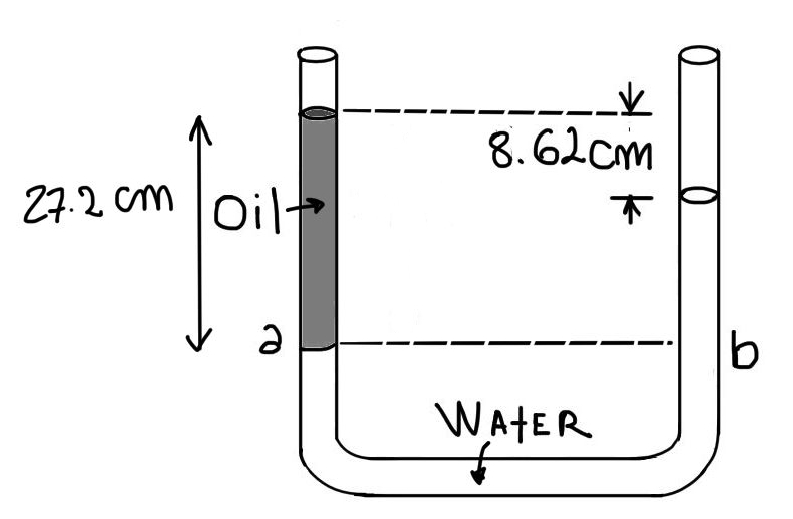
\includegraphics[height=1.5in]{images/2.jpg}
%   \end{center}
%   \caption{What is the density of the oil?}
% \end{figure}

A swimming pool is $5.0~m$ long, $4.0~m$ wide, and
$3.0~m$ deep. Compute the force exerted by the water against (a) the
bottom and (b) either end. (Hint: Calculate the force on a thin, horizontal
strip at a depth $h$, and integrate this over the end of the
pool.) Do not include the force due to air pressure. Density of water: $10^3~kg/m^3$



% First Section %%%%%%%%%%%%%%%%%%%%%%%%%%%%%%%%%%%%%%%%%%%%
\stepcounter{example}
\section*{Exercise \theexample (25 p)}

Take into account the speed of the top surface of the tank (Fig. \ref{image1}) and show that the speed of
fluid leaving the opening at the bottom is:

\begin{equation*}
  v_1=\sqrt{\frac{2gh}{(1-A^2_1/A^2_2)}}
\end{equation*}
where $h = y_2-y_1$, and $A_1$ and $A_2$ are the areas of the opening and of the top surface,
respectively. Find the distance $d$ at which the fluid reaches the floor.

\begin{figure}[h!]
  \begin{center}
    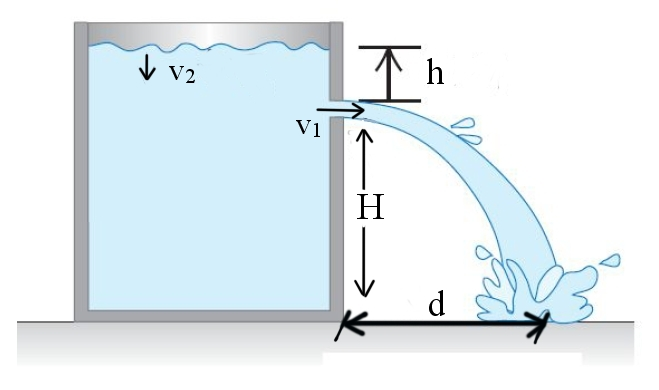
\includegraphics[height=2.in]{images/1.jpg}
  \end{center}
  \caption{Find $v_1$ and $d$}
  \label{image1}
\end{figure}

% First Section %%%%%%%%%%%%%%%%%%%%%%%%%%%%%%%%%%%%%%%%%%%%
\stepcounter{example}
\section*{Exercise \theexample (25 p)}

A student wants to use a meter stick as a pendulum.
She plans to drill a small hole through the meter stick
and suspend it from a smooth pin
attached to the wall (Fig. \ref{image3} ).
Where in the meter stick should
she drill the hole to obtain the
shortest possible period? How
short an oscillation period can she 
obtain with a meter stick in this
way? 
\vspace{2mm}

Inertia momentum of the stick respect to the center of mass: $\frac{1}{12}ML^2$


\begin{figure}[h!]
  \begin{center}
    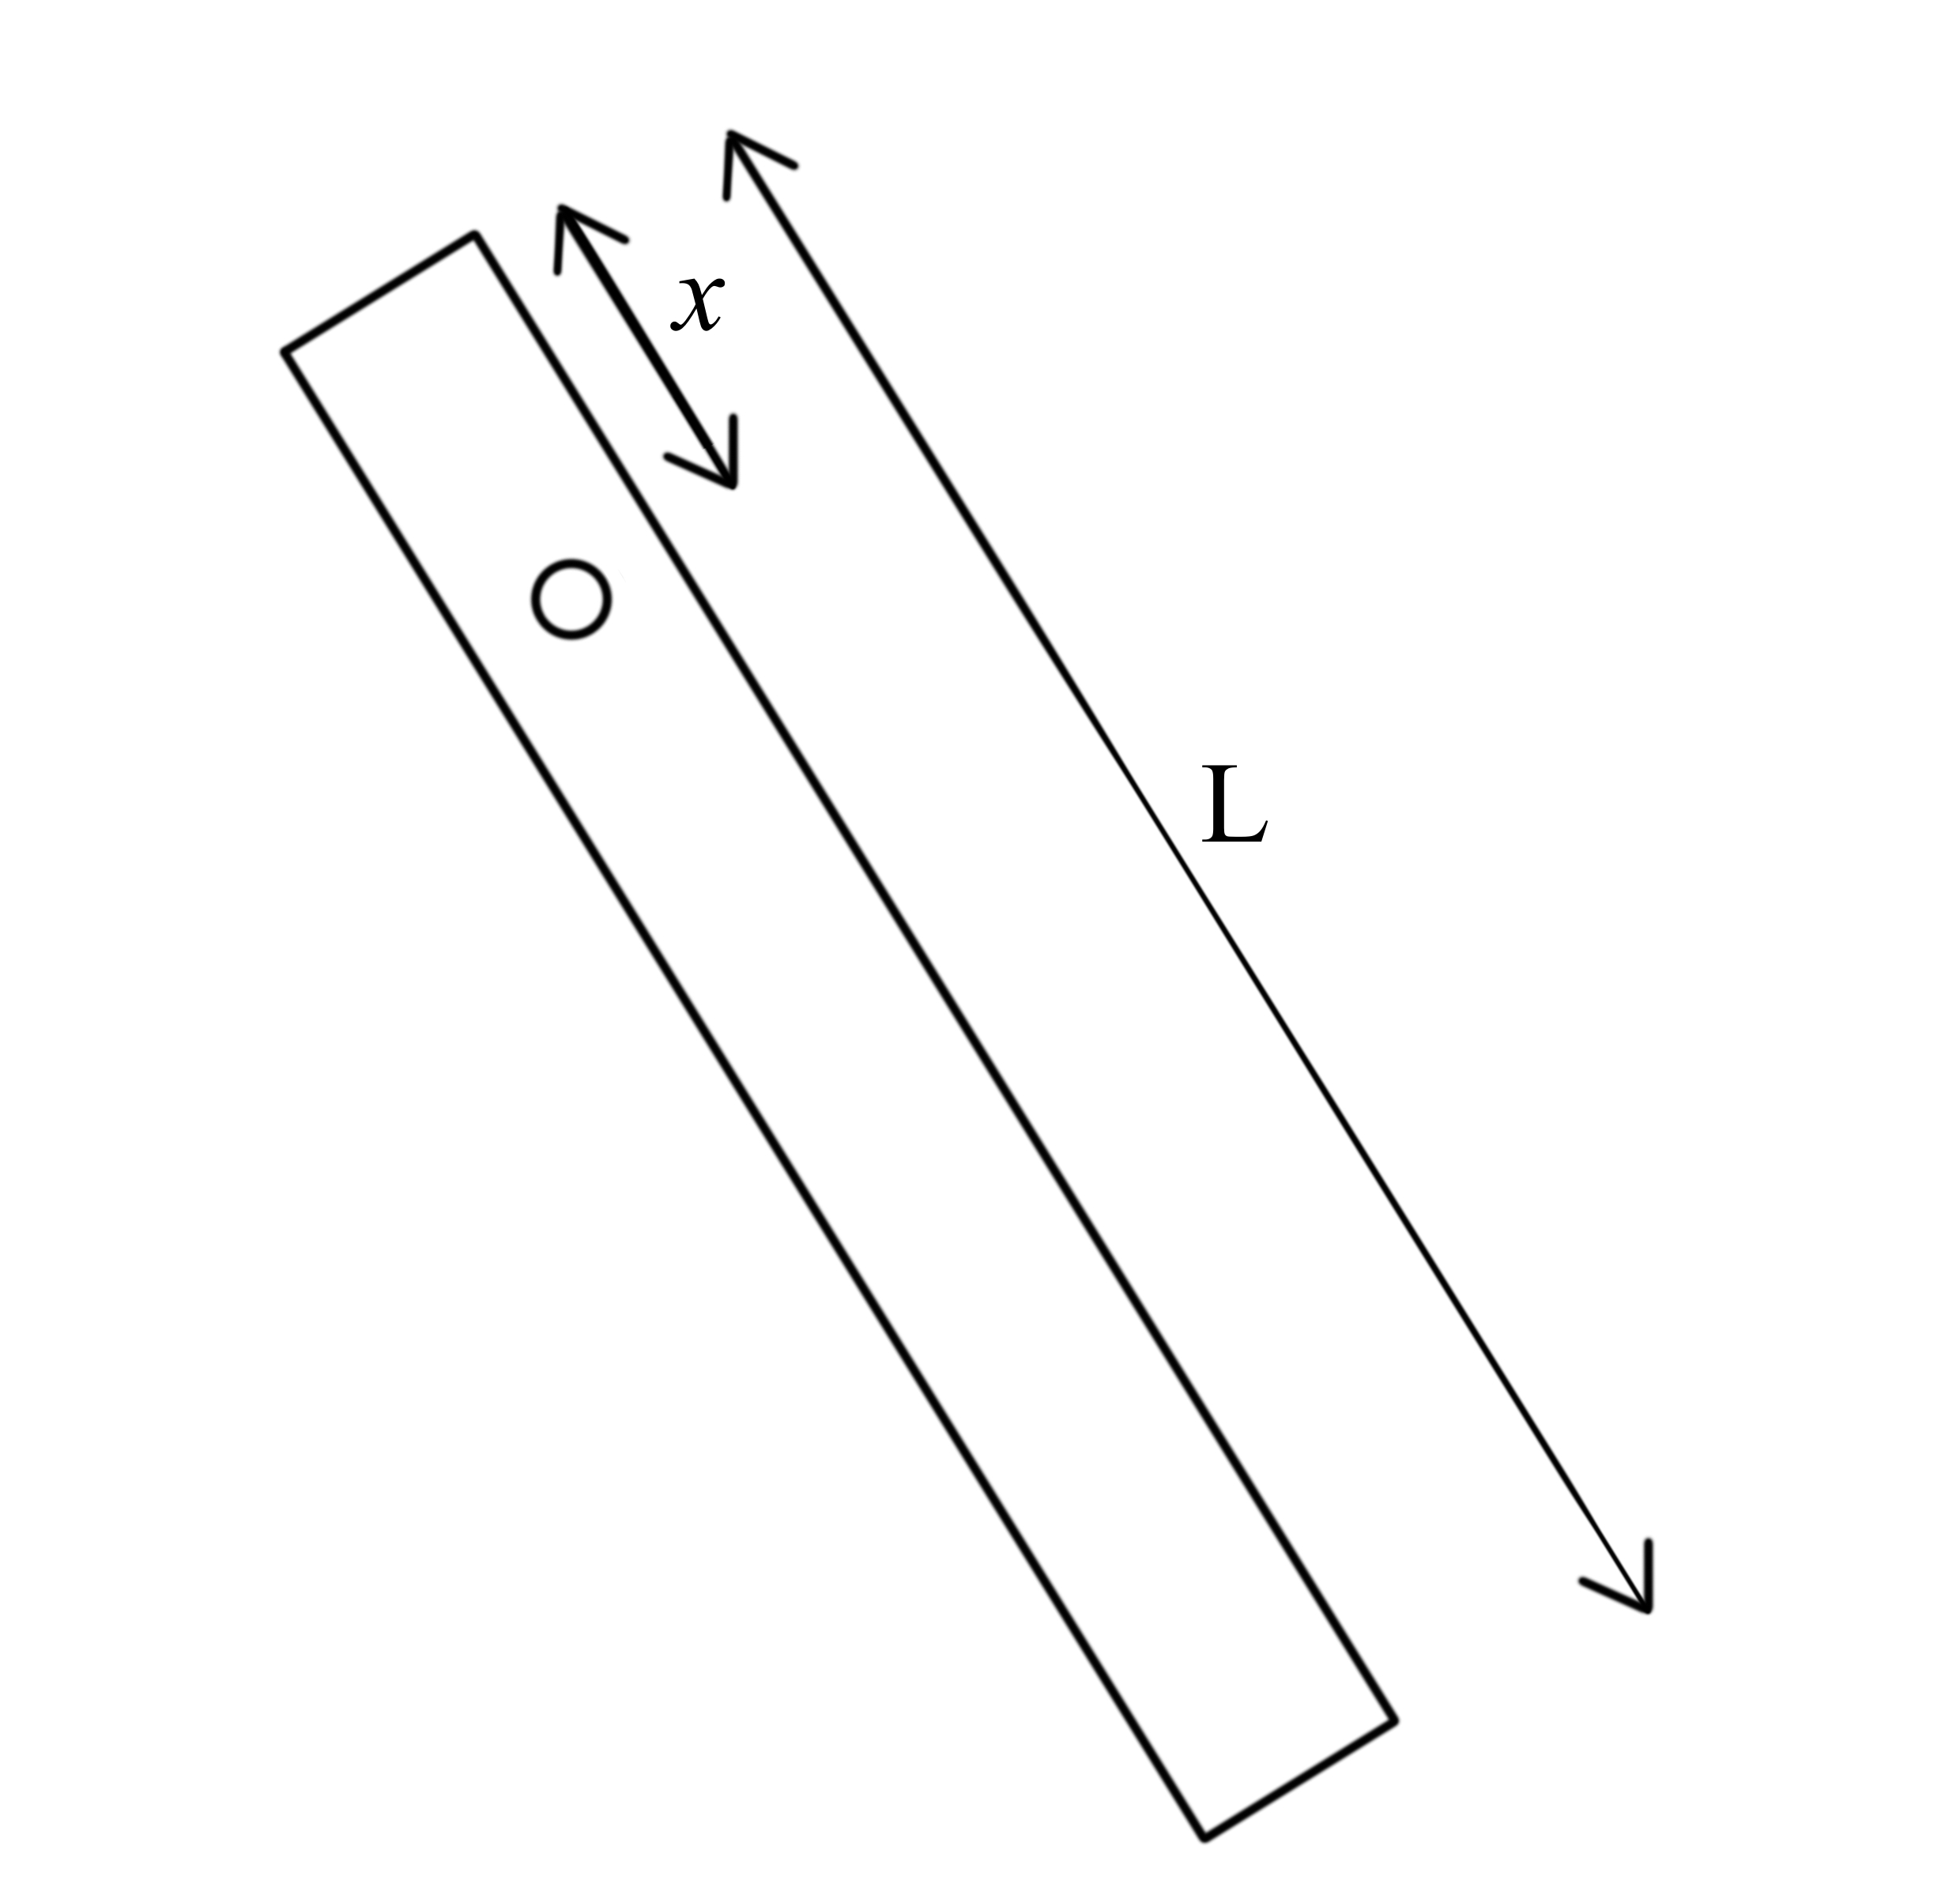
\includegraphics[height=2.2in]{images/3.jpg}
  \end{center}
  \caption{Find $x$ for the shortest period. }
  \label{image3}
\end{figure}


% First Section %%%%%%%%%%%%%%%%%%%%%%%%%%%%%%%%%%%%%%%%%%%%
% \stepcounter{example}
% \section*{Exercise \theexample}

% Three pieces of string, each of length $L$, are joined
% together end to end, to make a combined string of length $3L$. The
% first piece of string has mass per unit length $\mu_1$, the second piece
% has mass per unit length $\mu_2=4\mu_1$ and the third piece has mass
% per unit length $\mu_3=\mu_1/4$ (a) If the combined string is under tension
% $F$, how much time does it take a transverse wave to travel the
% entire length $3L$? Give your answer in terms of $L$, $F$, and $\mu_1$
% (b) Does your answer to part (a) depend on the order in which the
% three pieces are joined together? Explain.





% First Section %%%%%%%%%%%%%%%%%%%%%%%%%%%%%%%%%%%%%%%%%%%%
\stepcounter{example}
\section*{Exercise \theexample (25 p)}

A $65-cm$ guitar string is fixed at both ends. In the
frequency range between $1.0$ and $2.0 kHz$, the string is found
to resonate only at frequencies $1.2,1.5$, and $1.8 kHz$. What is
the speed of traveling waves on this string?


% First Section %%%%%%%%%%%%%%%%%%%%%%%%%%%%%%%%%%%%%%%%%%%%
\stepcounter{example}
\section*{EXTRA CREDIT: 5p}

The velocity of waves on a string is $96 m/s$. If the
frequency of standing waves is $445 Hz$, how far apart are the
two adjacent nodes?


\end{document}


